\documentclass[10pt,landscape]{article}
\usepackage[italian]{babel}
\usepackage[utf8]{inputenc}
\usepackage{multicol}
\usepackage{calc}
\usepackage{ifthen}
\usepackage[landscape]{geometry}
\usepackage{hyperref}
\usepackage{bookmark}
\usepackage{amsmath}
\usepackage{amssymb}
\usepackage{tabularx}
\usepackage{caption}
\usepackage{verbatim}
\usepackage{systeme}
\usepackage{nicefrac}
\usepackage{accents}
\usepackage{enumitem}
\usepackage[printwatermark]{xwatermark}
\usepackage{tikz}
\usetikzlibrary{calc,matrix}
\usepackage[compact]{titlesec}
\usepackage{microtype}
\usepackage[flushleft]{threeparttable}
\usepackage{textcomp}
\usepackage{pifont}
\usepackage{pgfplots}
\usepackage{float}
\usepackage{mathtools}
\usepackage{todonotes}
\usepackage{amsfonts}
\usepackage[ruled,vlined]{algorithm2e}
\usepackage{lastpage}
\usepackage{listings}

\geometry{top=.5in,left=.5in,right=.5in,bottom=.5in,headsep=0in}

% Turn off header and footer
\pagestyle{empty}

% Reduce size of \section e \subsection
\titleformat{\section}{\normalfont\large\bfseries}{\thesection}{1em}{}
\titleformat{\subsection}{\normalfont\normalsize\bfseries}{\thesubsection}{1em}{}
\titleformat{\subsubsection}{\normalfont\small\bfseries}{\thesubsection}{1em}{}
\titlespacing{\section}{0pt}{0ex}{-0.5ex}
\titlespacing{\subsection}{0pt}{0ex}{-0.5ex}
\titlespacing{\subsubsection}{0pt}{0ex}{-0.5ex}

% Define BibTeX command
\def\BibTeX{{\rm B\kern-.05em{\sc i\kern-.025em b}\kern-.08em
		T\kern-.1667em\lower.7ex\hbox{E}\kern-.125emX}}

% Don't print section numbers
\setcounter{secnumdepth}{0}


\setlength{\parindent}{0pt}
\setlength{\parskip}{0pt plus 0.5ex}

\setlist[itemize]{noitemsep, nolistsep}
\setlist[enumerate]{noitemsep, nolistsep}

% No algorithm numbering
\renewcommand{\thealgocf}{}
% do-while
\SetKwRepeat{Do}{do}{while}

\newcommand{\rarr}{\rightarrow}

\newcommand{\cmark}{\ding{51}}%
\newcommand{\xmark}{\ding{55}}%

\pagenumbering{arabic}
\pagestyle{fancy}
\fancyhead[R]{Page \thepage{} of \pageref{LastPage}}
\fancyhead[L]{}
\fancyfoot[C]{}
\renewcommand{\headrulewidth}{0pt}

\lstdefinelanguage{Alloy}
{
  % list of keywords
  morekeywords={
    assert, pred, all, no, lone, one, some, check, run,
    but, let, implies, not, iff, in, and, or, set, sig, Int, int,
    if, then, else, exactly, disj, fact, fun, module, abstract,
    extends, open, none, univ, iden, seq, String
  },
  sensitive=true,
  morecomment=[l]{//},
  morecomment=[l]{--},
  morecomment=[s]{/*}{*/}
}

\lstset{
	tabsize=2,
    basicstyle=\ttfamily\scriptsize,
    %upquote=true,
    %aboveskip={1.5\baselineskip},
    columns=fixed,
    showstringspaces=false,
    extendedchars=true,
    breaklines=true,
    prebreak = \raisebox{0ex}[0ex][0ex]{\ensuremath{\hookleftarrow}},
    %frame=single,
    %rulecolor=\color[rgb]{0.75,0.75,0.75},
    showtabs=false,
    showspaces=false,
    showstringspaces=false,
    keywordstyle=\color[rgb]{0,0,1},
    commentstyle=\color[rgb]{0.133,0.545,0.133},
    stringstyle=\color[rgb]{0.627,0.126,0.941},
    emphstyle={[1]\color[rgb]{0.133,0.545,0.133}},
}


\begin{document}

\raggedright
\footnotesize
\begin{multicols}{3}

% multicol parameters
% These lengths are set only within the two main columns
%\setlength{\columnseprule}{0.25pt}
\setlength{\premulticols}{1pt}
\setlength{\postmulticols}{1pt}
\setlength{\multicolsep}{1pt}
\setlength{\columnsep}{2pt}

{\Large{\textbf{Software Engineering 2}}}

\section{Alloy}
\lstinputlisting[language=Alloy]{2-alloy/alloy.als}

\section{World and Machine}
The \emph{machine} is the portion of system to be developed (software and hardware).
The \emph{world} (aka the environment) is the portion of the real world affected by the machine.

Phenomena can be \emph{shared} between world and machine.
Shared phenomena can be controlled by the machine and observed by the world, or viceversa.

\textbf{Goals} are prescriptive assertions formulated in terms of world phenomena.\\
\textbf{Domain assumptions} are descriptive assertions assumed to hold in the world.\\
\textbf{Requirements} are prescriptive assertions formulated in terms of shared phenomena.

Example of interaction betweem world and machine:
\todo[inline]{make this bigger}
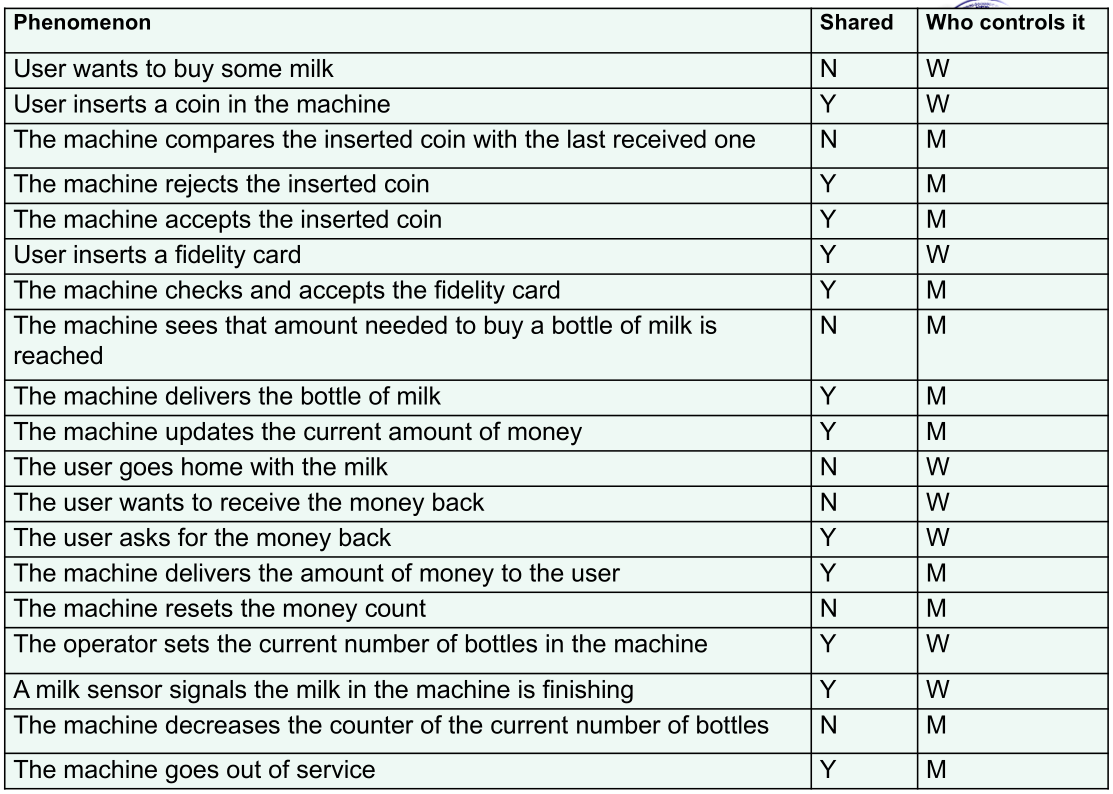
\includegraphics[width=\linewidth]{3-world-machine/shared-example.png}
\section{UML}
\subsection{Use case diagram}
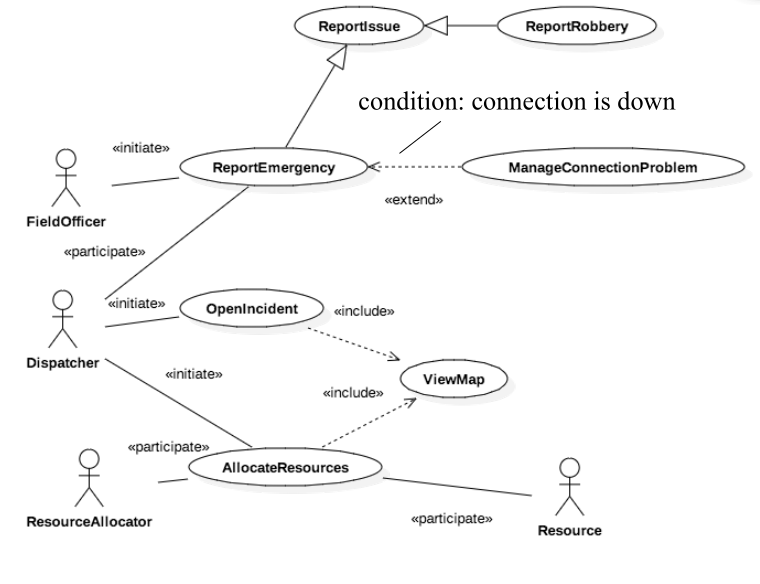
\includegraphics[width=\linewidth]{4-uml/use-case.png}

\subsection{Class diagram}
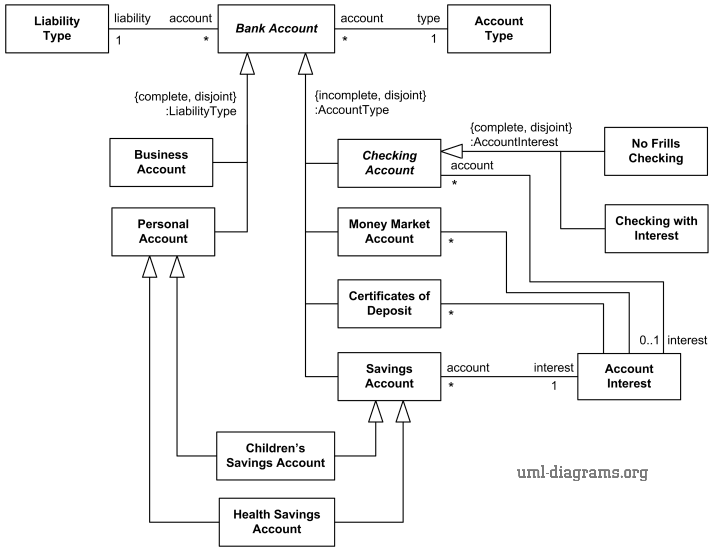
\includegraphics[width=\linewidth]{4-uml/class.png}

\subsection{Sequence diagram}
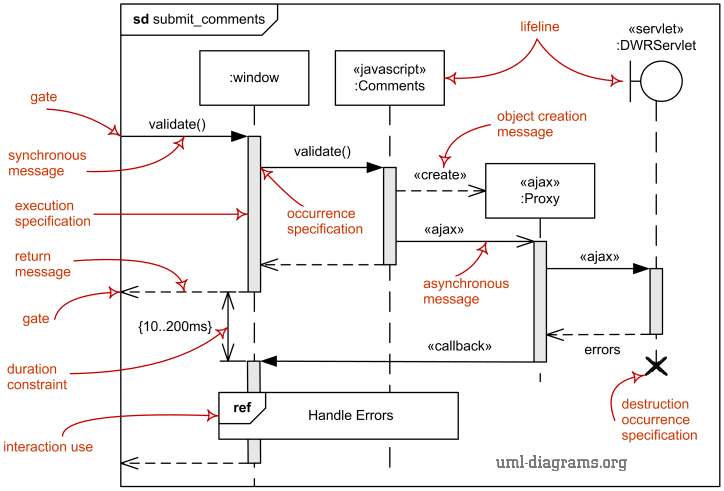
\includegraphics[width=\linewidth]{4-uml/sequence.png}

\subsection{State diagram}
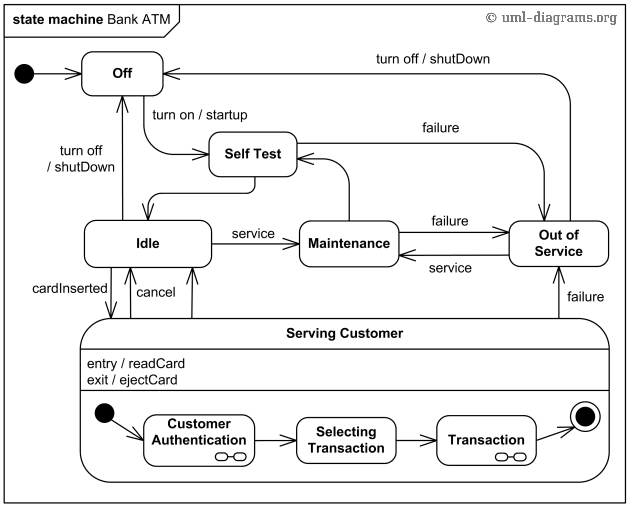
\includegraphics[width=\linewidth]{4-uml/state.png}

\subsection{Object diagram}
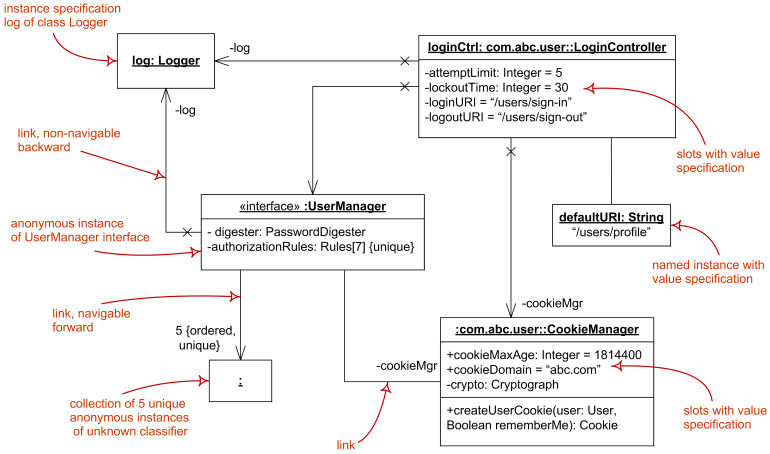
\includegraphics[width=\linewidth]{4-uml/object.png}

\subsection{Composite Structure diagram}
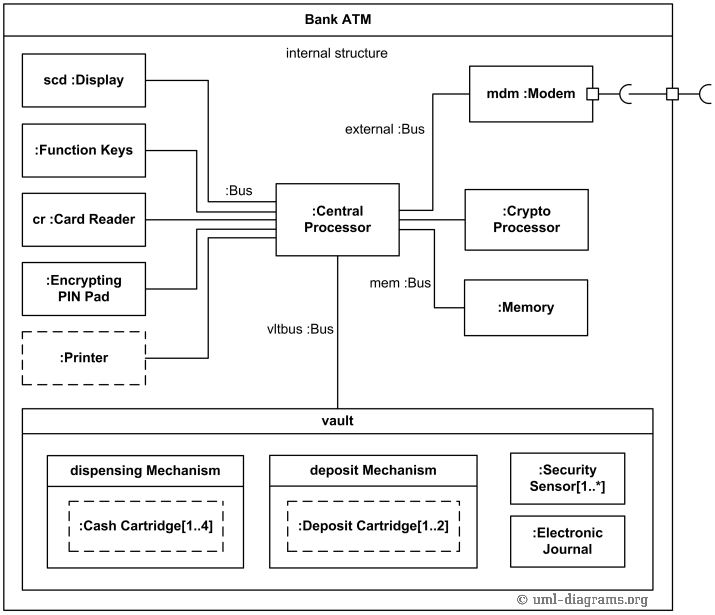
\includegraphics[width=\linewidth]{4-uml/composite.png}

\subsection{Component diagram}
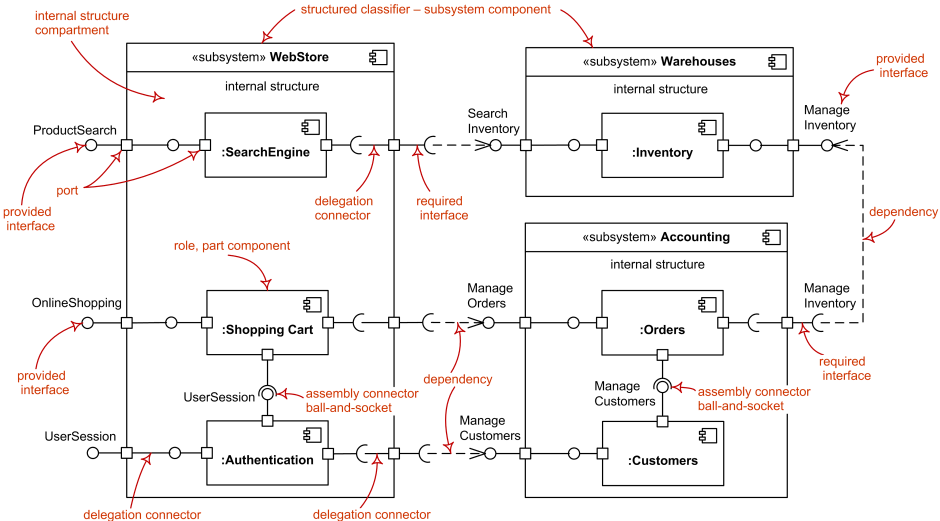
\includegraphics[width=\linewidth]{4-uml/component.png}

\subsection{Deployment diagram}
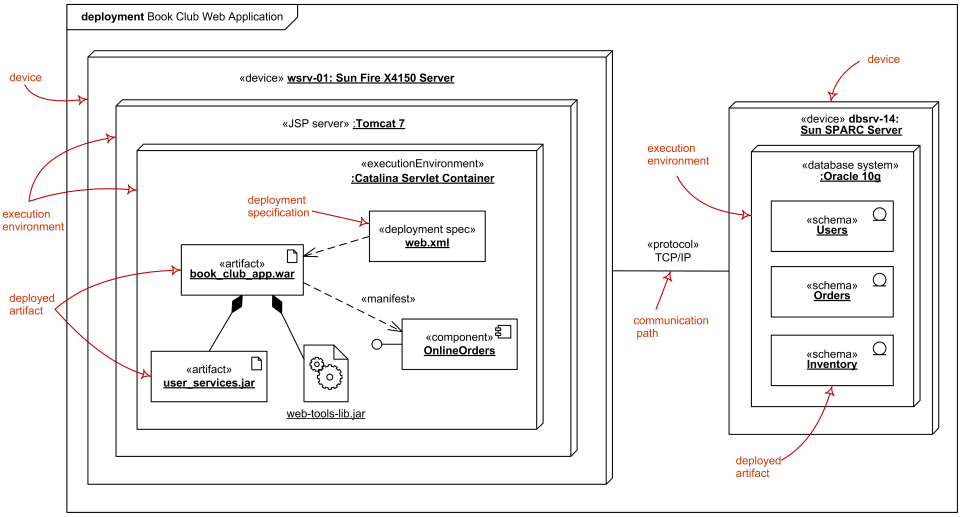
\includegraphics[width=\linewidth]{4-uml/deployment.png}
\section{Analysis of architectures}
\begin{minipage}{0.4\linewidth}
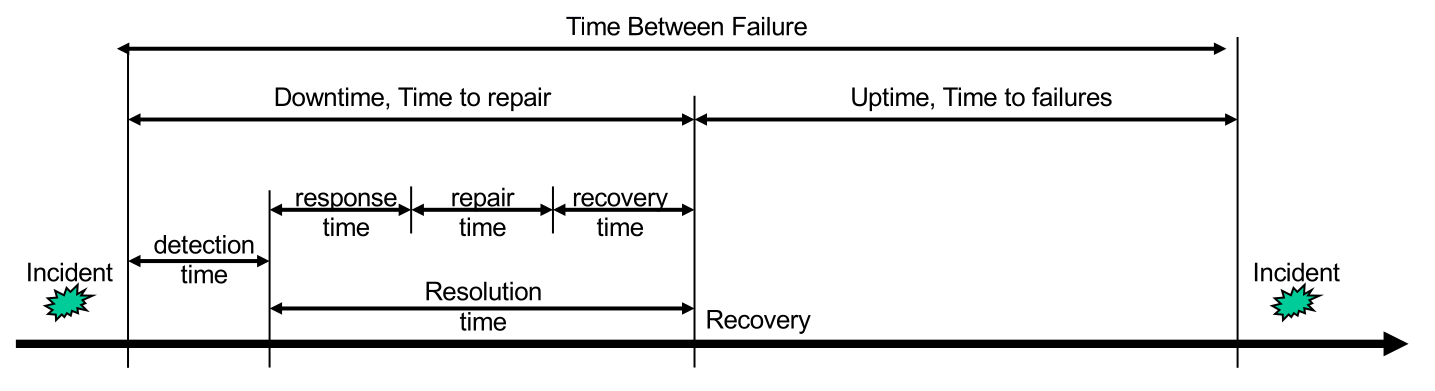
\includegraphics[angle=90, origin=c, width=\linewidth]{6-design/lifecycle-failure.png}
\end{minipage}
\begin{minipage}{0.58\linewidth}
\textbf{Time of occurence}: time at which the user becomes aware of the fault.\\
\textbf{Detection time}: the service provider is informed.\\
\textbf{Response time}: time required by the service provider to respond to the user.\\
\textbf{Repair time}: time required to restore the service or the component that caused the fault.\\
\textbf{Recovery time}: time required to restore the system.\\ \\
\textbf{Mean Time To Repair (MTTR)}: average time between the occurrence of a fault and recovery.\\
\textbf{Mean Time To Failures (MTTF)}: average time between the recovery of an incident and the occurence of the next one.\\
\textbf{Mean Time Between Failures (MTBF)}: average time between the occurrence of two consecutive faults.\\ \\

$MTBF = MTTR + MTTF$.
\end{minipage}

\subsection{Availability}
Probability that a component is working properly at a given time.
\[ A = \frac{MTTF}{MTTF + MTTR} \]

Availability in series: $A = \prod A_i$\\
Availability in parallel: $A = 1 - \prod (1 - A_i)$

\subsection{Reliability}
Probability that a component has always been working properly during a time interval $(0, t)$.
\[ R = e^{-\lambda t} \qquad \lambda =\frac{1}{MTTF} \]
\section{Testing and Verification}
\begin{itemize}
\item Verification: is the program right (correct)?
\item Validation: is the right program (what the client wants)?
\end{itemize}

Everything must be verified (specifications, design, test data etc.) along the entire development process.

Failures are usually result of faults introduced by human error.\\
Human Error → System fault → System failure

Verification and validation start as soon we decide to develop a product, design must permit testing of the system.

Difficulties:
\begin{itemize}
    \item Impossible to develop error free software
    \item Properties may bu subjective
    \item Properties may be implicit or not clearly stated
    \item Goals not reasonable
\end{itemize}

\subsection{Verification model}
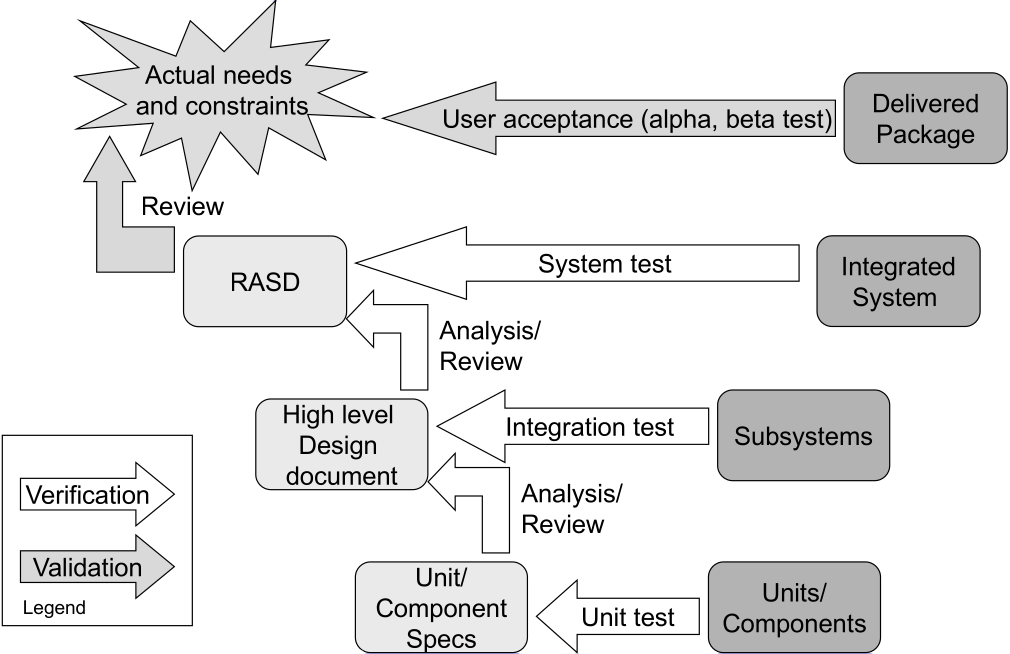
\includegraphics[width=\linewidth]{7-testing/v-model.png}

\section{Analysis}
Software is not executed, so analysis can be made even at early stages when software cannot be executable (yet).
The two main approaches are (manual) inspection and automated static analysis.

\subsection{Review, Walkthrough, Inspection}
Formal evaluation in which software (or plans, design, documentation, everything) is examined to find faults, violations of standards etc.

Objective is finding errors in the product, not fixing them or evaulting the producer.

\textbf{Walkthrough}
Producer presents product and the reviewers comment on the correctness and consistency.
\begin{itemize}
    \item Informal review
    \item Reviewers are experts in the domain
    \item Subject is correctness of product from POV of experts
    \item Leader of discussion/session controller is the producer
\end{itemize}

\textbf{Inspection}
\begin{itemize}
    \item Formal review
    \item Reviewers are trained, professional inspectors
    \item Subject is correctness of product according to given checklist
    \item Leader of discussion/session controller is official moderator of review team
\end{itemize}
Various roles:
\begin{itemize}
    \item Moderator: plans meeting, chooses participants, controls all the process
    \item Readers and testers (inspectors): read code and look for flaws
    \item Author: passive, only answer to questions
    \item Scribe (recorder)
\end{itemize}
Session are at most 2 hours, max 150 lines per hour.
Defects are only logged, not fixed.

\textbf{Modern code review}
Code visible to everyone, review facilitated by various tools.
Helps in exchanging and recording ideas.

\subsection{Static Analysis}
Based on identification of pairs of variables definitions and use.
Typically used by compilers to check for possible errors and to make optimizations.
Pessimistic approach, some problems may actually be false positives.
\begin{enumerate}
    \item Derive control flow graph
    \item Derive def and use sets for every node
    \item Identify pairs of def-use
\end{enumerate}

Can be used to check if variable is guaranteed to be initialized or if variable is never used.

\textbf{Symbolic execution}
Values are expressed over symbols, executing statements computes new expressions.
In case of branches, execution is performed only for a specified path.

\section{Testing}
\textbf{Test case} is a set of inputs of the system, along with the expected outcome (given hypothesis on state of the system).
\textbf{Test set} is a set of test cases.

Test cases can be generate randomly or systematically.

\subsection{Unit testing}
Conducted directly by the developers on single units of code.
Component may not work in isolation, so \emph{drivers} and \emph{stubs} are needed (this is called \textbf{scaffolding}).
Unit testing should be done as soon as possible.

\subsection{Integration testing}
Aimed to test interfaces and modules interactions.
Example of integration faults are:
\begin{itemize}
    \item Inconsistent interpretation of parameters
    \item Violations of capacity or size limits
    \item Side effects on resources
    \item Omitted or misunderstood functionality
    \item Nonfunctional properties (e.g. performance issues)
    \item Dynamic mismatches
\end{itemize}
Integration plan is an important part of the test plan, which is part of the project plan.

\textbf{Big Bang testing}\\
All integration testing done at the end, no scaffolding required.
Very bad, it has an high cost of repair (bugs found early cost less to be fixed).

\textbf{Incremental testing}\\
Integration testing is done while component are released, even at early stages.

\subsection{Testing strategies}
\begin{itemize}
    \item Top-down (requires stubs)
    \item Bottom-up (requires drivers)
    \item Thread (develop one function at a time)
    \item Critical modules (start by riskier modules, to verify feasibility)
\end{itemize}

\subsection{System testing}
Testing of the whole system, both functional and non-functional.
\begin{itemize}
    \item Performance testing (identify bottlenecks and benchmarking)
    \item Load testing (expose bugs such as memory leaks, identify upper limits of components)
    \item Stress testing (see how the system behaves in case of failures or sudden change of load and resources)
\end{itemize}

\subsection{Testing techniques}
\textbf{White box} Used usually for uni testing, based on knowledge of structure of the system.

\textbf{Black box} Used to test integration and the whole system. Used to check if expected behavior is the behavior of the software (\emph{Model-based testing}).

\textbf{Capture and reply} First test is manual (so it is costly) but it is recorded. Next time the test is an automatic replay of the first test, for which we know the outcome (used for example for auto-regression testing on GUI).
\section{Project Management}
A project is a temporary organization that has a specific and unique goal and usually a budget (costs, materials, resources).

Project Management is used to manage (plan, monitor, control) the scope, time and cost in order to make the project successful.

\section{Project management processes}
\begin{enumerate}
    \item Initiating
    \item Planning
    \item Executing
    \item Monitoring and controlling
    \item Closing
\end{enumerate}
\subsection{1. Initiating}
\begin{itemize}
    \item Define the project
    \item Define initial scope
    \item Estimate cost and resources
    \item Define the stakeholders
\end{itemize}

\subsection{2. Planning}
\begin{itemize}
    \item Scope management plan: defining, validating and controlling scope
    \item Schedule management plan: how schedule is developed, managed, executed and controlled
    \item Cost management plan
    \item Quality management plan: quality standards, quality assurance and control
    \item Change management plan
    \item Communication management plan
    \item Risk management plan: identify risks and plan responses
\end{itemize}

\subsubsection{Risk Management}
\textbf{Risk} is an uncertain event that if occurs can impact the achievement of objectives.
\begin{itemize}
    \item Risk cause: source (or driver) of the risk
    \item Risk event: uncertain event that might follow the cause
    \item Risk effect: how the objectives might be affected by the risk event
\end{itemize}
Steps for risk management:
\begin{enumerate}
    \item Define roles and responsibilities
    \item Identify possible risks
    \item Give probability (high, low, medium) to each risk
    \item Develop a risk response plan
    \item Define a budget for unknown risks
\end{enumerate}
Type of risks:
\begin{itemize}
    \item Project risks (threaten project plan)
    \item Technical risks (threaten quality and timeliness of product)
    \item Business risks (e.g. market risk, strategic risk, sales risk, management risk, budget risk)
\end{itemize}

\subsubsection{Schedule planning}
Tasks are activities which must be completed to achive the project goal.
Milestones are points in the schedule where progress can be assessed.
Deliverables are work products delivered to the customer (e.g documents).

\begin{enumerate}
    \item Break down project in tasks
    \item Define dependencies between tasks
    \item Define lag time between dependencies (even negative)
\end{enumerate}

\begin{center}
    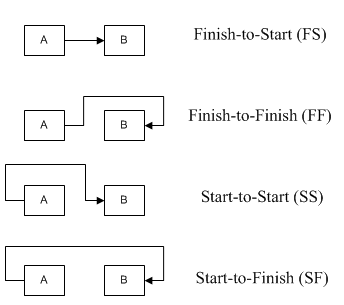
\includegraphics[width=0.6\linewidth]{8-project-management/tasks-dependencies.png}
\end{center}

The critical path is a sequence of tasks that runs from the start to the end of the project.
Changes to task on the critical path changes the project finish date.
A task is critical if it cannot float earlier or later.

Contraints can be:
\begin{itemize}
    \item Flexible (as soon as possible)
    \item Partial flexible (start no earlier than / finish no later than)
    \item Inflexible (must occur on specific time interval)
\end{itemize}

\subsubsection{Cost and Effort estimation}
Two types of techniques: experience-based techniques (based on past projects) and algorithmic cost modelling (formulaic approach).

Estimation changes based on number of COTS and components, programming language used, distribution of the team etc.
Exact size can only be known when project is finished.
\begin{center}
    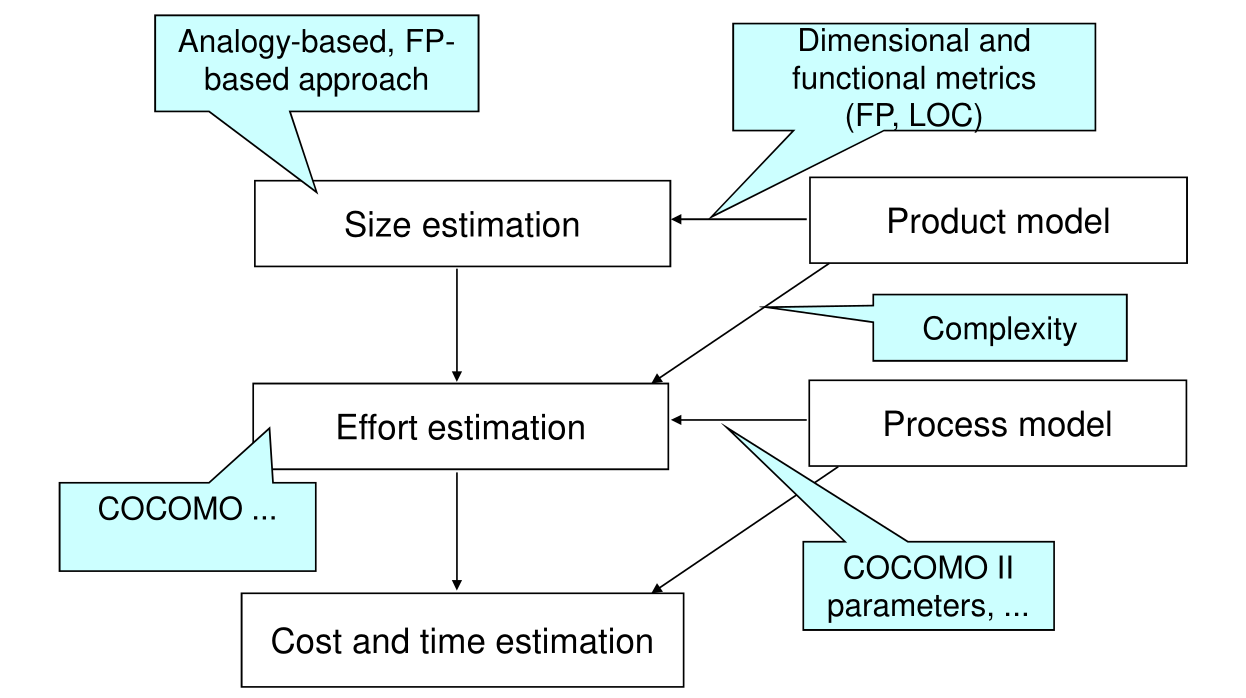
\includegraphics[width=\linewidth]{8-project-management/estimation.png}
\end{center}

\subsubsection{Function Points}
Characterize software dimension basing on functionalities.

Function types:
\begin{itemize}
    \item Internal Logical File (ILF): homogeneous set of data used and managed by the application.
    \item External Logical File (ELF): homogeneous set of data used by the application but maintained by others.
    \item External Input: elementary operation to elaborate date coming from external environment.
    \item External Output: elementary operation that generates data for the external environment (usually includes elaboration of LF).
    \item External Inquiry: elementary operation that involves input and output (without significant elaboration of LF).
\end{itemize}
Every function type is given a weight based on the complexity (simple, medium, complex).
The sum is the Unadjusted Function Points (UFP).
Function points can be used to estimate $LOC = AVC \cdot UFP$, where $AVC$ is language dependent.

\subsubsection{COCOMO II}
Two cases: \emph{Post-Architecture} (extension of existing product) or \emph{Early Design}.
\[ PM = A \cdot Size^E \prod EM_i \]
Where:
\begin{itemize}
    \item $PM$ is Person-Month
    \item $A = 2.94 \frac{PM}{KSLOC}$
    \item $Size$ is the estimated size of the project in $KSLOC$ (Kilo-Source Lines of Code)
    \item $EM$ is \emph{Effort Multiplier} (derived from \emph{Cost Drivers})
    \item $E$ is aggregation of five \emph{Scale Factors}
\end{itemize}

\textbf{Scale Factors}\\
\begin{itemize}
    \item Precedentedness: high if product is similar to previously developed projects.
    \item Dev. Flexibility: high if there are no specific constraints conform to pre-established requirements and external interface specs.
    \item Risk resolution: high if we have a good risk management plan, clear budget and schedule.
    \item Team cohesion: high if stakeholders are able to work in a team.
    \item Process maturity: refers to a well known method for assessing maturity of software organization (CMM, CMMI).
\end{itemize}
\todo[inline]{Make this bigger}
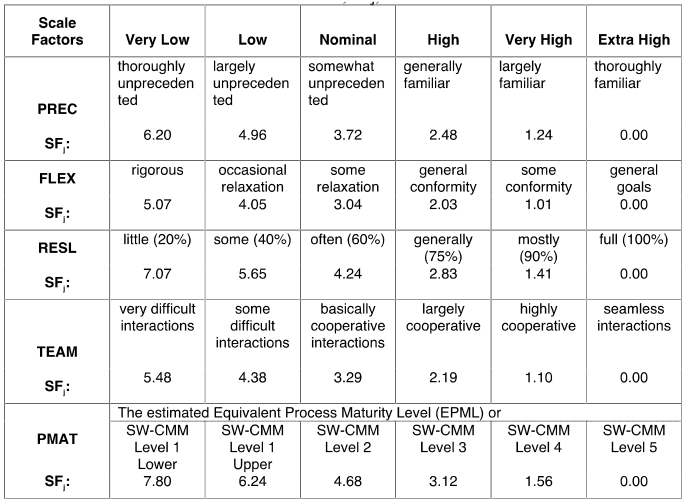
\includegraphics[width=\linewidth]{8-project-management/scale-factors.png}
\[ E = B + 0.01 \sum_{j=1}^{5} SF_j \qquad B = 0.91 \]

\textbf{Cost Drivers (Post-Architecture)}\\
\begin{itemize}
    \item Product Factors
    \begin{itemize}
        \item Required Software Reliability (RELY)
        \item Data Base Size (DATA)
        \item Product Complexity (CPLX)
        \item Developed for Reusability (RUSE)
        \item Documentation Match to Life-Cycle Needs (DOCU)
    \end{itemize}
    \item Platform Factors
    \begin{itemize}
        \item Execution Time Constraint (TIME)
        \item Main Storage Constraint (STOR)
        \item Platform Volatility (PVOL)
    \end{itemize}
    \item Personnel Factors
    \begin{itemize}
        \item Analyst Capability (ACAP)
        \item Programmer Capability (PCAP)
        \item Personnel Continuity (PCON)
        \item Applications Experience (APEX)
        \item Platform Experience (PLEX)
        \item Language and Tool Experience (LTEX)
    \end{itemize}
    \item Project Factors
    \begin{itemize}
        \item Use of Software Tools (TOOL)
        \item Multisite Development (SITE)
    \end{itemize}
    \item General Factor
    \begin{itemize}
        \item Required Development Schedule (SCED)
    \end{itemize}
\end{itemize}

\textbf{Cost Drivers (Early-design)}\\
\begin{itemize}
    \item PERS (ACAP, PCAP, PCON)
    \item RCPX (RELY, DATA, CPLX, DOCU)
    \item RUSE (RUSE)
    \item PDIF (TIME, STOR, PVOL)
    \item PREX (APEX, PLEX, LTEX)
    \item FCIL (TOOL, SITE)
    \item SCED (SCED)
\end{itemize}

\subsection{3. Executing}
\begin{itemize}
    \item Launch the project : kick off meeting
    \item Acquire and manage project team (internal and \item external resources)
    \item Acquire the required equipment and materials and external services
    \item Execute the plans (communication, change, quality)
    \item Perform the work identified in the WBS
    \item Perform controlling and monitoring activities
\end{itemize}

\subsection{4. Monitoring and Controlling}
Monitoring consists of collecting data about where the project stands, since projects never stick to the initial plans due to changes, problems, etc.
Controlling is where you implement corrections to get your project back on track.
Controlling increases risks factors.
If schedule is important you can use techniques like fast-tracking and crashing
If money is a priority you can reduce costs by reducing resources or overhead costs.
If the schedule, money and resources are not negotiable reduce scope eliminating the tasks associated with it.

\subsubsection{Earned Value Analysis}
\begin{itemize}
    \item Budget at completion (BAC): total budget for the project
    \item Planned value (PV): budgeted cost of work planned
    \item Earned value (EV): budgeted cost of work performed
    \item Actual cost (AC): actual cost for the completed work
\end{itemize}

Behind schedule if $EV < PV$.
Over budget if $EV < AC$.

\textbf{Schedule POV}\\
Schedule Variance: $SV = EV - PV$\\
Schedule Performance Index = $SPI = EV/PV$

\textbf{Cost POV}\\
Cost Variance: $CV = EV - AC$\\
Cost Performance Index = $CPI = EV/AC$

\textbf{Estimate at completion}\\
Spending at the same rate: $EAC = BAC/CPI$\\
Continue to spend at original rate: $EAC = AC + (BAC - EV)$\\
Both CPI and SPI influence remaining work: $EAC = [AC + (BAC - EV)] / (CPI \cdot SPI)$

\subsubsection{Fast Tracking}
Push tasks to occur faster than they would, by using negative lag time.

\subsubsection{Crashing}
Shorten the tasks on the critical path, usually increases costs.

\subsection{5. Closing}
\begin{itemize}
    \item Ensure project acceptance
    \item Track project performance
    \item Lessons learned
    \item Close contracts
    \item Release resources
\end{itemize}
\section{JEE}
Framework used to facilitate the development of Enterprise Application (EA).
Application based on JEE are portable everywhere there is Java EE.
JEE applications are based on the use of \emph{components} that communicate with each other.
Components are deployed inside \emph{containers}, which provide various services such as lifecycle management, lookup of other components and communication between components.

Multitiered architecture:
\begin{itemize}
    \item Client tier
    \item Web tier
    \item Business tier
    \item Enterprise Information System (EIS) tier
\end{itemize}

\subsection{Client Tier Containers}
\textbf{Applet container} to manage the execution of applets (web browser + Java plugin).

\textbf{Application client container} to manage the execution of application client components.

\subsection{Client Tier Components}
\textbf{Application client} is a component that runs directly on the machine.

\textbf{Applet} is a component that is integrated in a web page and executed through a plugin.

\textbf{Web clients} is a client made of dynamic web pages generated by web components (only browser needed).

\subsection{Web Tier Containers}
\textbf{Web container} is the interface between web components and the web server. Manages components lifecycle, dispatches requests to application components, provides information about current request.

\subsection{Web Tier Components}
\textbf{Servlets} is a component that extends the capabilities of a base server by using the request-response paradigm. Commonly used for HTTP requests. Acts as a middleware.

\textbf{JSP pages} text-based documents that embed JSP (Java) elements, that are dynamically constructed (dynamic content).

\textbf{JavaServer Pages} based on servlets and JSP, provides user interface component framework fro web applications.

\subsection{Business Tier Container}
\textbf{EJB container} provides a run-time environment for enterprise beans within the application. Middleware between business logic within the beans and the rest of the application server. Maintains pools of beans to improve performance and is a midddleware between beans and the underlying EIS.

\subsection{Business Tier Components}
\textbf{Enterprise Java Bean} is a server-side component that encapsulates the business logic of an application.
There are various types of beans:
\begin{itemize}
    \item Session beans
    \begin{itemize}
        \item Stateful session beans: one bean for each client, maintains state of the conversation.
        \item Stateless session beans: does not maintain any kind of state, all instances are equivalent.
        \item Singleton session beans: only one instance per application.
    \end{itemize}
    \item Message-driven beans: act as a JMS (Java Messaging System) message listener. These beans execute upon receiving a new message, stateless by design, all instances are equivalent.
\end{itemize}

\subsection{JNDI}
\emph{Java Naming and Directory Interface} enables components to locate other components and resources.
Each resource is identified by a unique identifier (JNDI name).

Generic lookup:
\begin{lstlisting}[language=Java]
DataSource ds = (DataSource) InitialContext
    .lookup("java:comp/DefaultDataSource");
\end{lstlisting}

\subsection{Resource Injection}
Another way to use JNDI names.
Injects JNDI resources directly, resolved by resource name and it is not type safe.
\begin{lstlisting}[language=Java]
public class MyServlet extends HttpServlet {
    @Resource(name="java:comp/DefaultDataSource")
    private javax.sql.DataSource dsc;
}
\end{lstlisting}

\subsection{Dependency Injection}
Java classes become managed objects.
Higher decoupling.
Injects regular classes, resolved by type, and it is type safe.
\begin{lstlisting}[language=Java]
public class Billing {
    @inject CurrencyConverter cc;
}
\end{lstlisting}

\subsection{Instance Pooling}
JEE maintains a pool of ready to use beans, in order to have better performance.
In case of stateless session beans or message-driven beans, every instance is the same (there is no state).
In this case beans can only have two states: \emph{ready} or \emph{non-existent}.

Lifecycle:
\begin{enumerate}
    \item Create bean.
    \item Dependency Injection.
    \item Invocation of \lstinline{@PostConstruct} method (if exists).
    The bean is now ready.
    \item When ready, the bean can accept various requests (or messages in case of message-driven beans).
    \item At the end of lifecycle, invocation of \lstinline{@PreDestroy} method (if exists).
    \item Bean is garbage-collected.
\end{enumerate}

In case of singleton beans, only one instance per application.
If singleton is annotated with \lstinline{@Startup}, it is instantiated upon application deployment.

\subsection{Activation/Passivation}
Used for stateful session beans.
Each bean, if not used, is serialized and written to disk (Passivation).
When a requests to that bean arrives, the bean is read from disk and recreated (Activation).

Lifecycle:
\begin{enumerate}
    \item Create bean.
    \item Dependency Injection.
    \item Invocation of \lstinline{@PostConstruct} method (if exists).
    The bean is now ready.
    \item When ready, the bean can accept various requests.
    \item For passivation, invocation to \lstinline{@PrePassivate}.
    \item For activation, invocation to \lstinline{@PostActivate}.
    \item At the end of lifecycle, invocation of \lstinline{@Remove}.
    \item Invocation of \lstinline{@PreDestroy} method (if exists).
    \item Bean is garbage-collected.
\end{enumerate}
%%%%%%%%%%%%%%%%%%%%%%%%%%%%%%%%%%%%%%%%%%%%%%%%%%%%%%%%%%%%%%%%%%%%%%%%%%%%%%%%
\vfill
\rule{\linewidth}{0.25pt}
\scriptsize\\
\href{mailto:marco.donadoni@mail.polimi.it}{M. Donadoni}, \href{mailto:edoardo.morassutto@mail.polimi.it}{E. Morassutto}, Politecnico di Milano, A.A. 2018/19
\end{multicols}

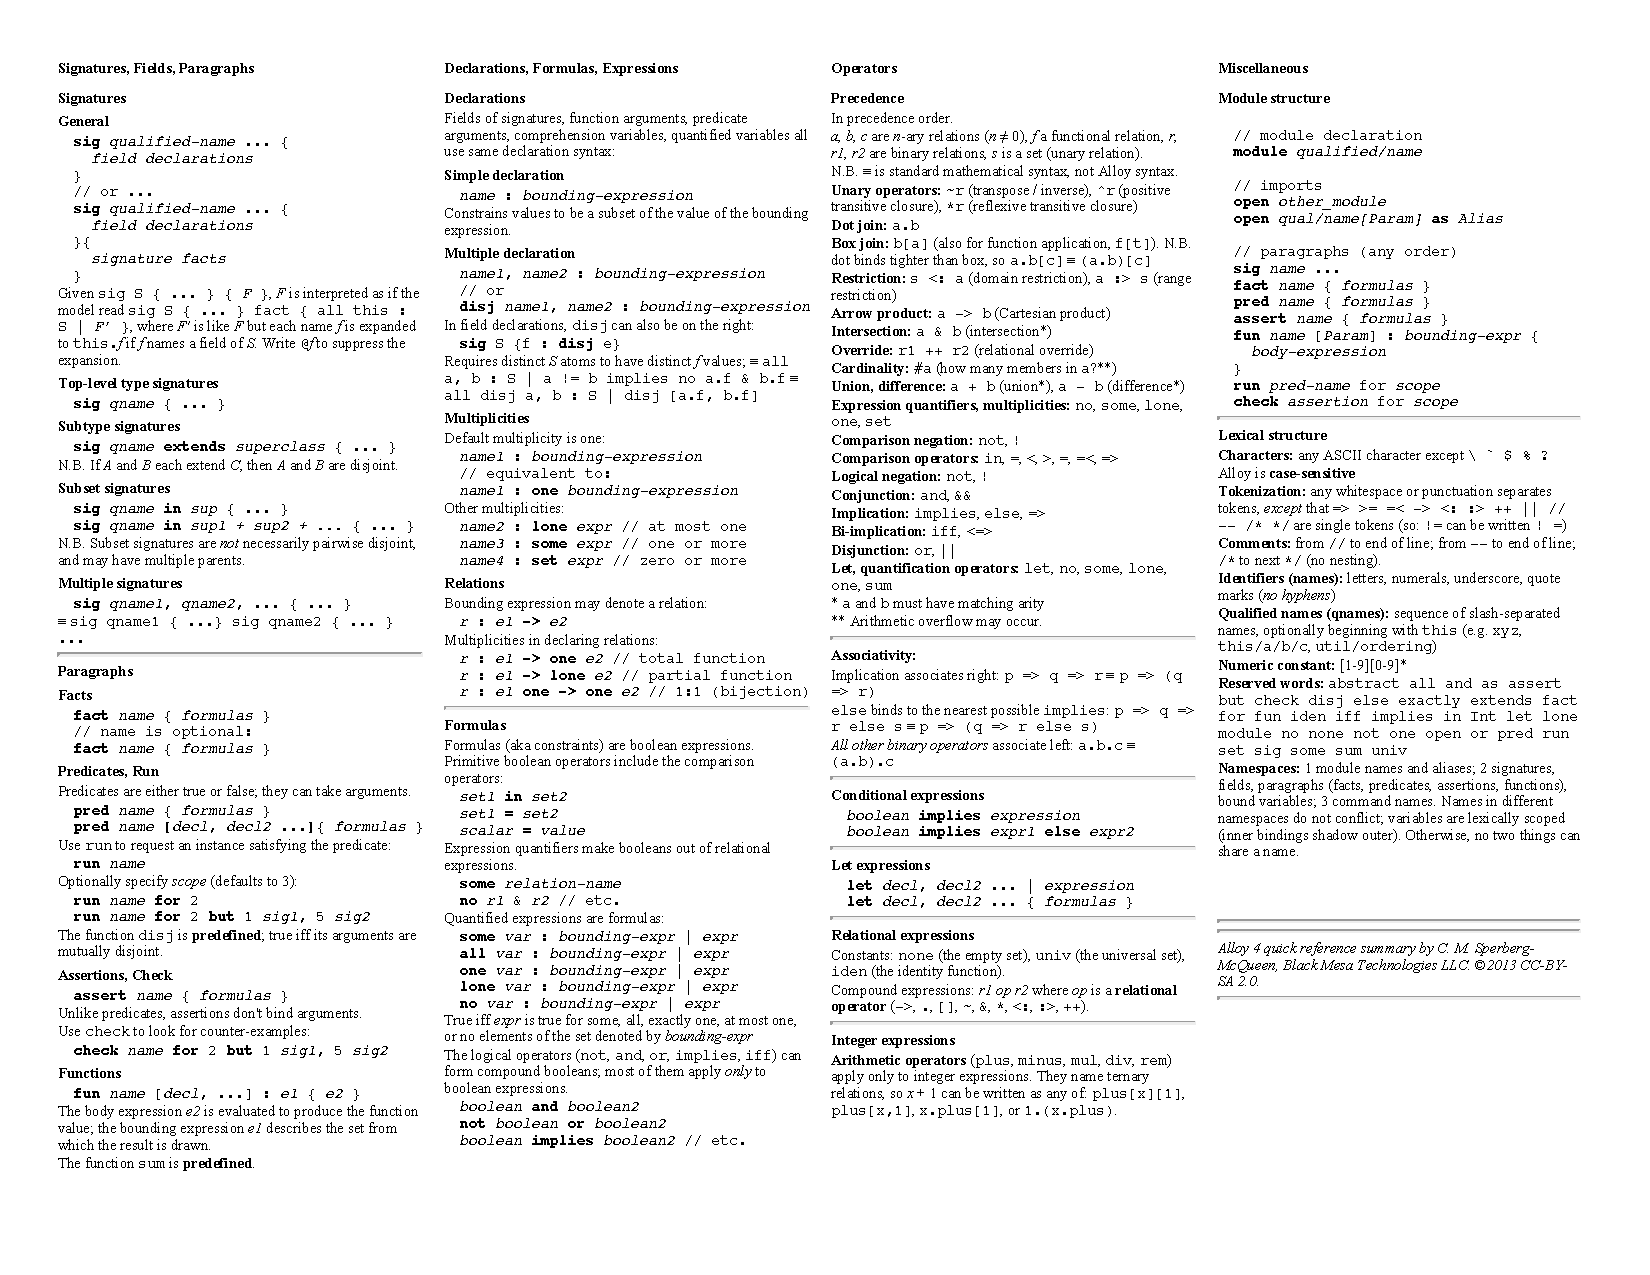
\includepdf[page=-]{alloy-cheatsheet.pdf}
\end{document}
